%%\documentclass[handout]{beamer}
%\documentclass[aspectratio=169,13pt]{beamer}

%\newcommand{\dee}{\partial}

\newcommand{\bmat}[1]{\begin{bmatrix} \B{#1}_{11} & \B{#1}_{12} \\ \B{#1}_{21} & \B{#1}_{22}\end{bmatrix}}
\newcommand{\blmat}[1]{\begin{bmatrix} \B{#1}_{11} &  \\ \B{#1}_{21} & \B{#1}_{22}\end{bmatrix}}
\newcommand{\brmat}[1]{\begin{bmatrix} \B{#1}_{11} & \B{#1}_{12} \\ & \B{#1}_{22}\end{bmatrix}}
\newcommand{\bomat}[1]{\begin{bmatrix} {#1}_{11} & \B{#1}_{12} \\ \B{#1}_{21} & \B{\uppercase{#1}}_{22}\end{bmatrix}}
\newcommand{\blomat}[1]{\begin{bmatrix} {#1}_{11} & \\ \B{#1}_{21} & \B{\uppercase{#1}}_{22}\end{bmatrix}}
\newcommand{\bromat}[1]{\begin{bmatrix} {#1}_{11} & \B{#1}_{12} \\  & \B{\uppercase{#1}}_{22}\end{bmatrix}}

\DeclareMathOperator{\vcop}{vec}
\newcommand{\vc}[1]{\vcop\left(#1\right)}
\newcommand{\prm}{\mu}

\newcommand{\fl}{fl}
\newcommand{\asmcond}[1]{\smallskip{\it #1}\smallskip}
\newcommand{\amdcond}[1]{\smallskip{\it #1}\smallskip}
\newcommand{\algcond}[1]{\smallskip{\it #1}\smallskip}
\newcommand{\atsmcond}[1]{{\it #1}}
\newcommand{\atmdcond}[1]{{\it #1}}
\newcommand{\atlgcond}[1]{{\it #1}}
\newcommand{\afillnum}[1]{{\underline{ \ #1\ \ }}}

\mode<presentation>
{
  \usetheme{Malmoe}
}

\usepackage[english]{babel}
%
%\usepackage[latin1]{inputenc}
%
%\usepackage{times}
%\usepackage[T1]{fontenc}
% Or whatever. Note that the encoding and the font should match. If T1
% does not look nice, try deleting the line with the fontenc.

\usepackage{inconsolata}
\usepackage{listings}
\usepackage{bm}
\usefonttheme[onlymath]{serif}
\renewcommand\familydefault{\sfdefault}
\usepackage[sfdefault]{ClearSans} %% option 'sfdefault' activates Clear Sans as the default text font
%\usefonttheme{professionalfonts}

\usepackage{latexsym}
\usepackage{amsmath}
\usepackage{amssymb}
\usepackage{amsfonts}
\usepackage{graphics}
\usepackage{multicol}

\definecolor{darkred}{rgb}{0.8,0.2,0.2}
\newcommand{\coloremph}[1]{\textcolor{darkred}{\emph{#1}}}        % colored italics
\newcommand{\reshape}[2]{o_{#1}(#2)}        % colored italics
\newcommand{\ket}[1]{\lvert #1 \rangle}
\newcommand{\bra}[1]{\langle #1 \vert}
\newcommand{\transp}[2]{{#2}^{\langle  {#1} \rangle }}        % colored italics

% Miscellaneous special math symbols

% Big-oh notation - either Latex's calligraphic O or uppercase math italic O
\newcommand{\BIGOH}{\mathcal{O}}                              % big oh
%\newcommand{\BIGOH}{O}                                       % big oh
\newcommand{\BIGTHETA}{\Theta}                                % big theta

\newcommand{\sfrac}[2]{{#1}/{#2}}

% Various versions of the fraction one-half
% solidus 1/2 for superscripts:
\newcommand{\SHALF}{1/2}                                      % one-half power
% small 1/2 set case in displayed equations:
\newcommand{\HALF}{\mbox{\small $\frac{1}{2}$}}               % small one-half
\newcommand{\THRD}{\mbox{\scriptsize $\frac{1}{3}$}}          % small one-third
\newcommand{\TWOTH}{\mbox{\scriptsize $\frac{2}{3}$}}         % small two-thirds

% Machine epsilon - note that placement of subscript may need adjustment.
%\newcommand{\emach}{\epsilon_{\textrm{\scriptsize mach}}} % machine prec.
\newcommand{\emach}{\epsilon}

\newcommand{\lsapprox}{\cong}                             % least squares approx

% Real numbers - Prefer \mathbb{R} but it requires amsfonts.
%                Latex's calligraphic R will do if amsfonts are unavailable.
%                DO NOT use \Re, which gives old German fraktur R.
\newcommand{\Real}{\mathbb{R}}                                 % real numbers
\newcommand{\Cplx}{\mathbb{C}}                                 % complex numbers
\newcommand{\Poly}{\mathbb{P}}                                 % polynomials
\newcommand{\Float}{\mathbb{F}}                                % fl pt system
% Bold math fonts for vectors and matrices
\renewcommand{\Vec}[1]{\ensuremath{\bm{#1}}}                   % vector
\newcommand{\Mat}[1]{\ensuremath{\bm{#1}}}                     % matrix
\newcommand{\Op}[1]{#1}                              % operator
\newcommand{\loc}[1]{x_{#1}}                              % operator

% Loglike functions set in regular type
\newcommand{\diag}{\mathrm{diag}}                             % diagonal matrix
\newcommand{\cond}{\mathrm{cond}}                             % condition number
\newcommand{\sign}{\mathrm{sign}}                             % sign function
\newcommand{\Span}{\text{span}}                             % span of matrix
%\newcommand{\trace}{\mathrm{trace}}                           % trace of matrix
\DeclareMathOperator*{\trace}{trace}
\newcommand{\tentrace}[3]{\trace_{#1,#2}(#3)}
\renewcommand{\Re}{\mathrm{Re}}                               % real part
\renewcommand{\Im}{\mathrm{Im}}                               % imaginary part

% Fractions appearing in matrices - allows setting them case or solidus
%\newcommand{\mf}[2]{{#1 \over #2}}        % matrix fraction - set case
\newcommand{\mf}[2]{#1/#2}               % matrix fraction - set solidus


% Keywords for algorithm statements

\newcommand{\FOR}{\textbf{for}\ }
\newcommand{\TO}{\textbf{to}\ }
\newcommand{\IF}{\textbf{if}\ }
\newcommand{\THEN}{\textbf{then}\ }
\newcommand{\ELSE}{\textbf{else}\ }
\newcommand{\WHILE}{\textbf{while}\ }
\newcommand{\DO}{\textbf{do}\ }
\newcommand{\BEGIN}{\textbf{begin}\ }
\newcommand{\END}{\textbf{end}\ }
\newcommand{\STOP}{\textbf{stop}\ }
\newcommand{\AND}{\textbf{and}\ }
\newcommand{\OR}{\textbf{or}\ }

\newcommand{\comm}{\mathrm{comm}}
\newcommand{\comp}{\mathrm{comp}}
\newcommand{\idle}{\mathrm{idle}}
\newcommand{\msg}{\mathrm{msg}}
\newcommand{\len}{\mathrm{s}}
\newcommand{\route}{\mathrm{route}}
\newcommand{\mitem}{\medskip\item}
\newcommand{\sitem}{\smallskip\item}
\DeclareMathOperator*{\argmin}{argmin}

%Gets rid of headline

\setbeamertemplate{footline}{}

\setbeamertemplate{headline}{}
\beamertemplatenavigationsymbolsempty



\definecolor{mygreen}{rgb}{0,0.2,0}
\definecolor{mygray}{rgb}{0.5,0.5,0.5}
\definecolor{mymauve}{rgb}{0.58,0,0.82}
\definecolor{mypurple}{rgb}{0.38,0,0.32}
\definecolor{myblue}{rgb}{0.2,0,0.5}
\definecolor{darkgreen}{rgb}{0.2,0.6,0.2}
\definecolor{Brown}{rgb}{0.39, 0.09, 0.0}
\definecolor{Violet}{rgb}{0.38, 0.0, 0.63}
\definecolor{myvlgray}{rgb}{0.9,0.9,1.0}
\definecolor{mylgray}{rgb}{0.85,0.85,0.9}
\definecolor{darkgreen}{rgb}{0,0.4,0}
\definecolor{brown}{rgb}{.6,.1,.1}

\newcommand{\bemph}[1]{{\color{blue} \emph{#1}}}

\usepackage{mathtools}
\newcommand{\defeq}{\coloneqq}

\newcommand{\inti}[2]{[{#1},{#2}]}
\newcommand{\BF}{\mathbf}
\newcommand{\CF}{\mathcal}
\newcommand{\B}[1]{\bm{#1}}
\newcommand{\E}[1]{\bm{#1}}
\newcommand{\dis}{\displaystyle}
\newcommand{\lt}{\left}
\newcommand{\rt}{\right}

\newcommand{\cs}{H}

\DeclareMathOperator*{\rank}{rank}
\DeclareMathOperator*{\vecn}{vec}
\DeclareMathOperator*{\vecs}{vech}

\usepackage{eso-pic}
\newcommand{\cornertext}[1]{
  \AddToShipoutPictureFG*{
    \AtPageUpperLeft{\put(0,-10){\makebox[\paperwidth][r]{#1}}}  
   }%
}
\newcommand{\cornertexttwo}[2]{
  \AddToShipoutPictureFG*{
    \AtPageUpperLeft{\put(0,-10){\makebox[\paperwidth][r]{#1}}}  
    \AtPageUpperLeft{\put(0,-20){\makebox[\paperwidth][r]{#2}}}  
   }%
}
\newcommand{\linkdemo}[2]{{\footnotesize\href{https://relate.cs.illinois.edu/course/cs450-f18/f/demos/upload/#1/#2.html}{\color{Violet}{\it\textbf{Demo:} #2}\ }}}
\newcommand{\linkinclass}[2]{{\footnotesize\href{https://relate.cs.illinois.edu/course/cs450-f18/flow/#1/start/}{\color{darkgreen}{\it\textbf{Activity:} #2}\ }}}
\newcommand{\urcornerlinkinclass}[2]{\cornertext{\linkinclass{#1}{#2}}}
\newcommand{\dblurcornerlinkinclass}[4]{\cornertexttwo{\linkinclass{#1}{#2}}{\linkinclass{#3}{#4}}}
\newcommand{\urcornerlinkdemo}[2]{\cornertext{\linkdemo{#1}{#2}}}
\newcommand{\dblurcornerlinkdemo}[4]{\cornertexttwo{\linkdemo{#1}{#2}}{\linkdemo{#3}{#4}}}
\newcommand{\urcornerlinkdemoinclass}[4]{\cornertexttwo{\linkdemo{#1}{#2}}{\linkinclass{#3}{#4}}}



% CS 554 specific:

\newcommand{\tsync}{\alpha}
\newcommand{\tword}{\beta}
\newcommand{\tflop}{\gamma}

\newcommand{\bw}{w}

\newcommand{\tpl}[2]{{\bm{#1}}}
\newcommand{\vtpl}[3]{{\bm{#1}}_#3}
\newcommand{\perm}[2]{\lt[#1\rt]_{#2}}
\newcommand{\costyle}{\ttfamily\bfseries}
\newcommand{\cotext}[1]{{\costyle{#1}}}
\newcommand{\kwstyle}{\costyle\textcolor{mypurple}}
\newcommand{\kwtext}[1]{{\kwstyle{#1}}}
\newcommand{\emstyle}{\costyle\textcolor{myblue}}
\newcommand{\emtext}[1]{{\emstyle{#1}}}
\newcommand{\const}{}
\newcommand{\work}{Q}
\newcommand{\depth}{D}
\newcommand{\flops}{F}
\newcommand{\words}{W}
\newcommand{\syncs}{S}
\newcommand{\mem}{M}
\newcommand{\eff}{E}
\newcommand{\isofun}[1]{\tilde{\work}(p)}
\newcommand{\isomem}[1]{\tilde{\mem}(p)}
\newcommand{\pstrong}{p_s}
\newcommand{\pweak}{p_w}
\newcommand{\ALL}{\star }
\newcommand{\rmn}[2]{\mathbb{R}^{#1\times #2}}
\newcommand{\rn}[1]{\mathbb{R}^{#1}}
\newcommand{\err}{\varepsilon}
\newcommand{\mat}[1]{\begin{bmatrix} #1 \end{bmatrix}}
\newcommand{\mc}[1]{\mathcal{#1}}
\newcommand{\h}[2]{\mc{H}_{#1}(#2)}
\newcommand{\T}{T}%{\mathsf{T}}
\newcommand{\dn}[2]{\mc{M}_{#1}^{\uparrow}(#2)}
%\usepackage[colorlinks=false,urlbordercolor={1.0 1.0 1.0}]{hyperref}
%
%\lstset{ %
%  postbreak=false,
%%  backgroundcolor=\color{white},   % choose the background color; you must add \usepackage{color} or \usepackage{xcolor}
%  basicstyle=\costyle,        % the size of the fonts that are used for the code
%%  breakatwhitespace=false,         % sets if automatic breaks should only happen at whitespace
%%  breaklines=false,                 % sets automatic line breaking
%  captionpos=n,                    % sets the caption-position to bottom
%  commentstyle=\color{mygreen},    % comment style
%  deletekeywords={...},            % if you want to delete keywords from the given language
%  escapeinside={\%*}{*)},          % if you want to add LaTeX within your code
%  extendedchars=true,              % lets you use non-ASCII characters; for 8-bits encodings only, does not work with UTF-8
%  frame=none,                    % adds a frame around the code
%  keepspaces=true,                 % keeps spaces in text, useful for keeping indentation of code (possibly needs columns=flexible)
%  keywordstyle=\color{mypurple},       % keyword style
%  language=C++,                 % the language of the code
%  otherkeywords={*,...},            % if you want to add more keywords to the set
%  numbers=none,                    % where to put the line-numbers; possible values are (none, left, right)
%  numbersep=5pt,                   % how far the line-numbers are from the code
%  numberstyle=\tiny\color{mygray}, % the style that is used for the line-numbers
%  rulecolor=\color{black},         % if not set, the frame-color may be changed on line-breaks within not-black text (e.g. comments (green here))
%  showspaces=false,                % show spaces everywhere adding particular underscores; it overrides 'showstringspaces'
%  showstringspaces=false,          % underline spaces within strings only
%  showtabs=false,                  % show tabs within strings adding particular underscores
%  stepnumber=2,                    % the step between two line-numbers. If it's 1, each line will be numbered
%  stringstyle=\color{mymauve},     % string literal style
%  tabsize=2,                     % sets default tabsize to 2 spaces
%  title=\lstname,                   % show the filename of files included with \lstinputlisting; also try caption instead of title
%  keywordstyle=\emstyle
%}

\lstset{ %
  postbreak=false,
%  backgroundcolor=\color{white},   % choose the background color; you must add \usepackage{color} or \usepackage{xcolor}
  basicstyle=\footnotesize\costyle,        % the size of the fonts that are used for the code
%  breakatwhitespace=false,         % sets if automatic breaks should only happen at whitespace
%  breaklines=false,                 % sets automatic line breaking
  captionpos=n,                    % sets the caption-position to bottom
  commentstyle=\color{mygreen},    % comment style
  deletekeywords={privatei,shared},            % if you want to delete keywords from the given language
  escapeinside={\%*}{*)},          % if you want to add LaTeX within your code
  extendedchars=true,              % lets you use non-ASCII characters; for 8-bits encodings only, does not work with UTF-8
  frame=none,                    % adds a frame around the code
  keepspaces=true,                 % keeps spaces in text, useful for keeping indentation of code (possibly needs columns=flexible)
  keywordstyle=\footnotesize\color{mypurple},       % keyword style
  language=C++,                 % the language of the code
  otherkeywords={*,pragma},            % if you want to add more keywords to the set
  numbers=none,                    % where to put the line-numbers; possible values are (none, left, right)
  numbersep=5pt,                   % how far the line-numbers are from the code
  numberstyle=\footnotesize\color{mygray}, % the style that is used for the line-numbers
  rulecolor=\color{black},         % if not set, the frame-color may be changed on line-breaks within not-black text (e.g. comments (green here))
  showspaces=false,                % show spaces everywhere adding particular underscores; it overrides 'showstringspaces'
  showstringspaces=false,          % underline spaces within strings only
  showtabs=false,                  % show tabs within strings adding particular underscores
  stepnumber=2,                    % the step between two line-numbers. If it's 1, each line will be numbered
  stringstyle=\footnotesize\color{mymauve},     % string literal style
  tabsize=2,                     % sets default tabsize to 2 spaces
  title=\lstname,                   % show the filename of files included with \lstinputlisting; also try caption instead of title
  emph={MPI_Send,MPI_Recv,MPI_Comm,MPI_Comm_rank,MPI_Send,MPI_Comm_split,MPI_Init,MPI_Finalize,MPI_Status,MPI_COMM_WORLD,MPI_Datatype,MPI_Comm_size,MPI_FLOAT,mpi.h,omp,parallel,shared,private,default,reduction},
  emphstyle=\footnotesize\emstyle
}

\title{CS 450: Numerical Anlaysis\footnote{{\it These slides have been drafted by Edgar Solomonik as lecture templates and supplementary material for the book ``Scientific Computing: An Introductory Survey'' by Michael T. Heath (\href{http://heath.cs.illinois.edu/scicomp/notes/index.html}{{\color{blue} slides}}).}}}
\author{}
\institute{University of Illinois at Urbana-Champaign}




\subtitle{Partial Differential Equations}

\date{}
\begin{document}

\begin{frame}
  \titlepage
\end{frame}

\section{Types and Applications of PDEs}
\begin{frame}{Partial Differential Equations}

\begin{itemize}
\item \coloremph{Partial differential equations (PDEs)} describe physical laws and other continuous phenomena:

\lgcond{
\begin{itemize}
\item They contain partial derivatives in multiple variables.
\mitem Examples include: electromagnetism, fluid flow, quantum mechanics, and general relativity.
\end{itemize}
}

\item The \coloremph{advection PDE} describes basic phenomena in fluid flow,
\[u_t = -a(t,x)u_x\]
where $u_t=\dee u/\dee t$ and $u_x=\dee u/\dee x$.

\lgcond{
\begin{itemize}
\item Generally, we impose an initial condition with respect to $t$, i.e., $u(0,x)=u_0(x)$.
\mitem \coloremph{Boundary conditions} are also often exposed on boundary of domain.
\mitem When $a(t,x)=c$ this is the \coloremph{Cauchy problem} with solution,
\[u(t,x)=u_0(x-ct).\]
\end{itemize}
}

\end{itemize}
\end{frame}

\begin{frame}{Types of PDEs}
\urcornerlinkdemo{11-sparse-matrices-pdes}{Time-dependent PDEs}

\begin{itemize}
\item Some of the most important PDEs are \coloremph{second order}:

\lgcond{
\begin{itemize}
\item Heat equation (diffusion), $u_t=u_{xx}$
\item Wave equation (oscillation), $u_{tt}=u_{xx}$
\item Laplace equation (steady-state), $u_{xx}+u_{yy}=0$
\end{itemize}
Any PDE of the form
\[au_{xx}+bu_{xy}+cu_{yy}+du_x+eu_y+fu+g=0\]
behaves (has the character) of one of the above equations.
}

\item The \coloremph{discriminant} determines the canonical form of second-order PDEs:

\lgcond{
The discriminant is $r=b^2-4ac$ and linear PDEs are classified as
\[\begin{cases} 
  r>0 &: \text{\coloremph{hyperbolic}, wave-equation-like} \\
  r=0 &: \text{\coloremph{parabolic}, heat-equation-like} \\
  r<0 &: \text{\coloremph{elliptic}, Laplace-equation-like} 
  \end{cases} \]
When coefficients are varying, a PDE may exhibit different behavior in different parts of the domain.
%These cases are insufficient to describe all PDEs (higher order and systems of PDEs can be very different), 
%This characterization of the behavior (which may be different in different parts of the domain) of the bulk of typical PDE problems.
}

\end{itemize}

\end{frame}

\section{Hyperbolic and Parabolic PDEs}
\subsection{Characteristics}
\begin{frame}{Characteristic Curves}

\begin{itemize}
\item A \coloremph{characteristic} of a PDE is a level curve in the solution:
\lgcond{
\begin{itemize}
\item For the Cauchy form of the advection equation, $u_t=-cu_x$, a characteristic $\hat{x}(t)$ satisfies $u(t,\hat{x}(t))=\text{const}$.
\mitem One of their uses is identifying where boundary conditions must be imposed, e.g. for the Cauchy equation, it tells us whether boundary conditions are needed on the left or the right (in terms of $x$) of the domain.
\end{itemize}
}
\item More generally, characteristic curves describe curves in the solution field $u(t,x)$ that correspond to solutions of ODEs, e.g. for $u_t = -a(t,x)u_x$ with $u(0,x)=u_0(x)$,
\lgcond{
\[\hat{x}'(t) = -a(t,\hat{x}(t)) \text{ with initial condition } \hat{x}(0)=x_0.\]
These characteristic curves give solutions $\hat{u}(t,x)=u_0(\hat{x}(t))$, which satisfy the advection PDE $u_t = -a(t,x)u_x$, since 
\[\hat{u}_t =\hat{x}'(t)u_0'(\hat{x}(t)) = -a(t,x)u_0'(\hat{x}(t)) = -a(t,x)\hat{u}_x.\]
%$u_x^{(0)}(\hat{x}(t))a(t,\hat{x}(t))=a(t,x)u_0'(h\hat{x}(t))$
}
\end{itemize}

%\item The order of a PDE is the highest-order of any partial derivative appearing in the PDE:
%
%\lgcond{
%\begin{itemize}
%\item The advection equation is a first order PDE.
%\mitem PDEs containing e.g. $u_{xy}$ or $u_{tt}$ are second order.
%\end{itemize}
%}
%\end{itemize}

\end{frame}

\subsection{Semidiscrete Methods}

\begin{frame}{Method of Lines}


\begin{itemize}
\item \coloremph{Semidiscrete methods} obtain an approximation to the PDE by solving a system of ODEs.
      Consider the heat equation,
      \[u_t = cu_{xx} \text{ on } 0 \leq x \leq 1, \quad u(0,x)=f(x), u(t,0)=u(t,1)=0.\]
\vspace*{-.2in}
\lgcond{
\begin{itemize}
\item
We discretize over $x$ and use finite differences to approximate 
\[u_{xx} \approx  \frac{u(t,x_{i+1}) - 2u(t,x_i) + u(t,x_{i-1})}{(\Delta x)^2}.\]
\item
This approximation yields a system of ODE IVPs, where $y_i(t)\approx u(t,x_i)$,
\[y'_i(t) = \frac{c}{(\Delta x)^2}\Big(y_{i+1}(t) - 2y_{i}(t) + y_{i-1}(t)\Big), \quad y_i(0) = f(x_i).\]
\item
In vector form, we obtain a linear constant-coefficient ODE, 
\(\B y'(t) = \B A \B y(t),\)
where $\B A$ is tridiagonal.
\end{itemize}
% with $a_{ii} = -2, a_{i,i+1}=a_{i+1,i}=1$.
}
\smcond{}
\item This \coloremph{method of lines} often yields a stiff ODE:

\mdcond{
\begin{itemize}
\item
The eigenvalues of $\B A$ are in $[-4c/(\Delta x)^2,0]$, which gives stiff ODE for $\Delta x\ll 1$.
\sitem 
Heat dissipates very rapidly when concentrated, but slowly overall.
\end{itemize}
}

\end{itemize}



\end{frame}


\begin{frame}{Semidiscrete Collocation}

\begin{itemize}
\item Instead of finite-differences, we can express $u(t,x)$ in a spatial basis $\phi_1(x),\ldots,\phi_n(x)$ with time-dependent coefficients $\alpha_1(t),\ldots,\alpha_n(t)$:

\lgcond{
\[u(t,x) \approx v(t,x,\B \alpha(t)) = \sum_{j=1}^n \alpha_j(t) \phi_j(x)\]
\coloremph{Semidiscrete collocation} methods then ensure the approximation is exact on $x_1,\ldots, x_n$, yielding system of ODEs.
}

\item For the heat equation $u_t=cu_{xx}$, we obtain a linear constant-coefficient vector ODE:

\lgcond{
\[\sum_{j=1}^n \frac{\dee \alpha_j}{\dee t}(t)\underbrace{\phi_j(x_i)}_{m_{ij}} = c \sum_{j=1}^n \alpha_j(t)\underbrace{\frac{\dee^2 \phi_j}{\dee x^2}(x_i)}_{n_{ij}}\]
written in matrix form,
\[\B \alpha'(t) = c\B M^{-1} \B N\B \alpha(t)\]
}

\end{itemize}


\end{frame}

\subsection{Fully Discrete Methods for PDEs}

\begin{frame}{Fully Discrete Methods}

\begin{itemize}
\item Generally, both time and space dimensions are discretized, either by applying an ODE solver to a semidiscrete method or using finite differences.

\begin{itemize}
\atsmcond{
\item
Again consider the heat equation $u_t=c u_{xx}$ and discretize so $u^{(k)}_i \approx u(t_k,x_i)$,
}
\lgcond{
\[\frac{u_i^{(k+1)} - u_i^{(k)}}{\Delta t} = c\frac{u_{i+1}^{(k)}-2u_i^{(k)}+u^{(k)}_{i-1}}{(\Delta x)^2}.\]
}
\atsmcond{
\item This iterative scheme corresponds to a 3-point \coloremph{stencil},
}
\lgcond{
\[u_i^{(k+1)} = u_i^{(k)} + c\Delta t\frac{u_{i+1}^{(k)}-2u_i^{(k)}+u^{(k)}_{i-1}}{(\Delta x)^2}.\]
\item
The same scheme can be derived by applying Euler's method to the ODE given by the method of lines.
}
\end{itemize}
\lgcond{}

\end{itemize}

\end{frame}

\begin{frame}{Implicit Fully Discrete Methods}

\begin{itemize}
\item Using Euler's method for the heat equation, stability requirement is
\tmdcond{
\[\Delta t=O\big((\Delta x)^2\big)\]
}
\item This step-size restriction on stability can be circumvented by use of implicit time-stepper, such as backward Euler,
\tmdcond{
\[u_i^{(k+1)} = u_i^{(k)} + c\Delta t\frac{u_{i+1}^{(k+1)}-2u_i^{(k+1)}+u^{(k+1)}_{i-1}}{(\Delta x)^2}.\]
This scheme requires for a tridiagonal matrix system to be solved at each time-step, but obtains unconditional stability, albeit only first-order accuracy.
}
\item Using the trapezoid method to solve the ODE we obtain the second-order \coloremph{Crank-Nicolson method},
\tmdcond{
\[u_i^{(k+1)} = u_i^{(k)} + c\Delta t\frac{u_{i+1}^{(k+1)}-2u_i^{(k+1)}+u^{(k+1)}_{i-1}+u_{i+1}^{(k)}-2u_i^{(k)}+u^{(k)}_{i-1}}{2(\Delta x)^2}.\]
}
\end{itemize}

\end{frame}

\subsection{Convergence Criteria}

\begin{frame}{Convergence and Stability}

\begin{itemize}
\item \coloremph{Lax Equivalence Theorem}: consistency + stability = convergence

\algcond{
\begin{itemize}
\item
Consistency means that the local truncation error goes to zero, and is easy to verify by Taylor expansions.
\mitem
Stability implies that the approximate solution at any time $t$ must remain bounded.
\mitem
Together these conditions are necessary and sufficient for convergence.
\end{itemize}
}

\item Stability can be ascertained by spectral or Fourier analysis:

\algcond{

\begin{itemize}
\item
In the method of lines, we saw that the eigenvalues of the resulting ODE define the stability region.
\mitem
Fourier analysis decomposes the solution into a sum of harmonic functions and bounds their amplitudes.
\end{itemize}
}
\end{itemize}
\end{frame}



\begin{frame}{CFL Condition}

\begin{itemize}
\item The domain of dependence of a PDE for a given point $(t,x)$ is the portion of the problem domain influencing this point through the PDE:

\lgcond{
\begin{itemize}
\item
Generally determined by characteristics of PDE.
\mitem
For a stencil method, the numerical solution depends on the set of mesh-points influencing the mesh point at $(t,x)$.
\end{itemize}
}

\item \coloremph{The Courant, Friedrichs, and Lewy (CFL) condition} states that for an explicit finite-differencing scheme to be stable for a hyperbolic PDE, it is necessary that the domain of the dependence of the PDE must be contained in the domain of dependence of the scheme:

\lgcond{
Intuitively, we can then achieve stability for fixed $\Delta t$ in two ways,
\begin{itemize}
\mitem by choosing a sufficiently large grid spacing $\Delta x$, or 
\mitem including more mesh points in our stencil.
\end{itemize}
}

\end{itemize}
\end{frame}

\section{Elliptic PDEs}

\subsection{Discretization}

\begin{frame}{Time-Independent PDEs}

\begin{itemize}
\item We now turn our focus to time-independent PDEs as exemplified by the \coloremph{Helmholtz equation}:
\[u_{xx} + u_{yy} +\lambda u = f(x,y)\]

\lgcond{
\begin{itemize}
\item $\lambda=0$ yields the Poisson equation.
\mitem $\lambda=0$ and $f=0$ yields the Laplace equation.
\mitem Boundary conditions (e.g. Dirichlet or Neumann or mixed) are imposed on domain surface.
\end{itemize}
}

\item We discretize as before, but no longer perform time stepping:

\lgcond{
For example given a domain $[0,1]^2$, we can 
\begin{itemize}
\sitem tile it using $n\times n$ mesh points, 
\mitem setup finite-difference equations on interior,
\mitem setup boundary-condition equations on perimeter.
\end{itemize}
}

\end{itemize}
\end{frame}

\begin{frame}{Finite-Differencing for Poisson}

\begin{itemize}
\item Consider the Poisson equation with equispaced mesh-points on $[0,1]$:

\lgcond{
\begin{itemize}
\item
If $\B u$ is a vector containing the mesh-points, we have that
\[\mathcal{D}_x \B u + \mathcal{D}_y \B u = \B b \text{ where } b_i=f(u_i)\]
where $\mathcal{D}_x$ and $\mathcal{D}_y$ are finite-difference operators along $x$ and $y$ dimensions, respectively.
\mitem
Given a differencing matrix $\B D$ (e.g. tridiagonal with $1,-2,1$), we obtain the matrix equation,
\[(\B I \otimes \B D + \B D \otimes \B I)\B u = \B b\]
where the \coloremph{Kronecker product} is defined as 
\[\B C = \B A \otimes \B B = \begin{bmatrix} a_{11} \B B & a_{12} \B B & \cdots \\ a_{21} \B B & \ddots & \\ \vdots & & \end{bmatrix},\]
and the elements of $\B b$ contain the mesh elements in column-major (or row-major in this example) order.
\end{itemize}
}
\lgcond{}


\end{itemize}
\end{frame}









\begin{frame}{Multidimensional Finite Elements}

\begin{itemize}
\item There are many ways to define localized basis functions, for example in the 2D FEM method\footnote{\tiny Source: Comsol Multiphysics Cyclopedia \url{https://www.comsol.com/multiphysics/finite-element-method}}:

{

\centering

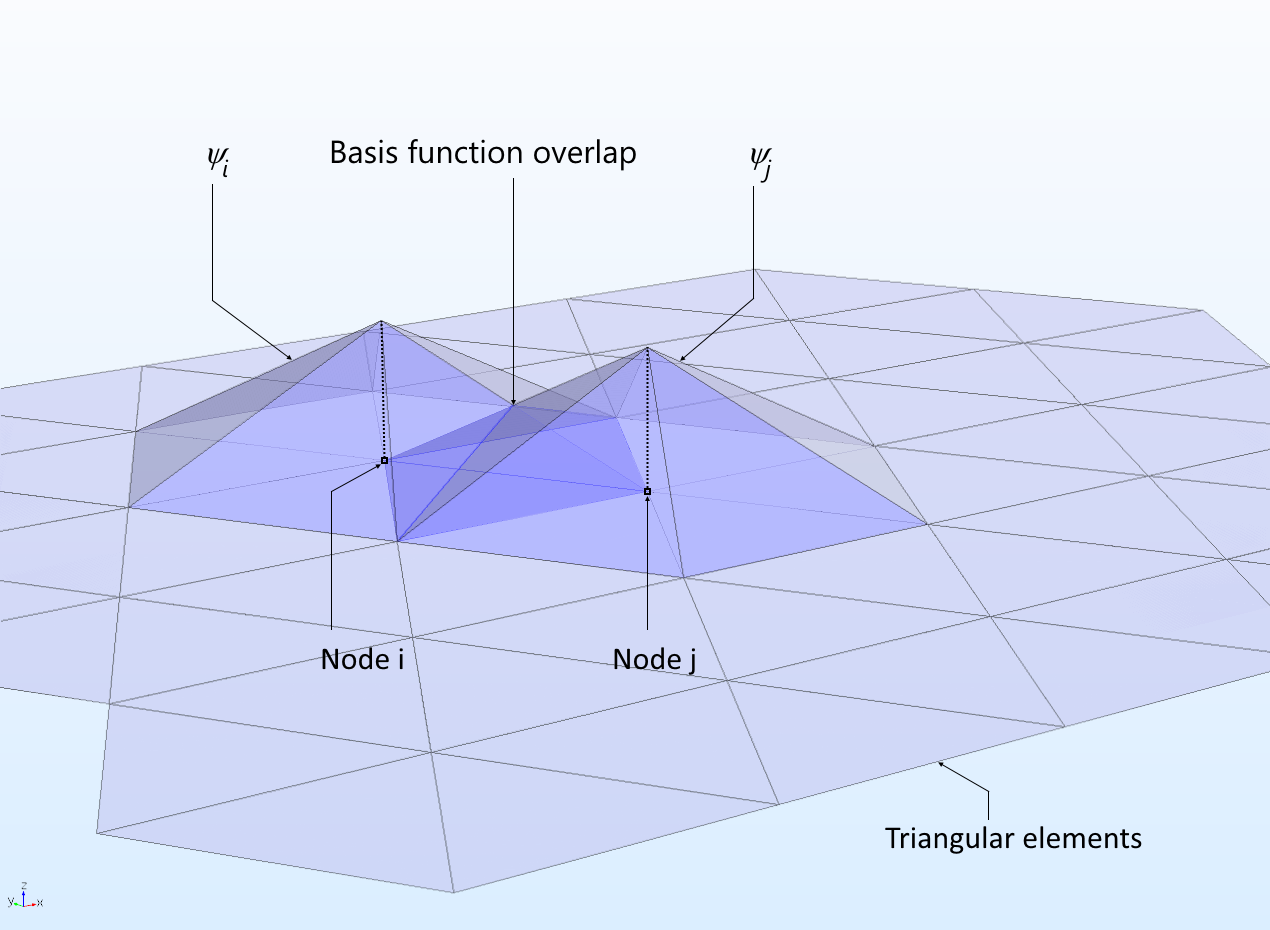
\includegraphics[width=2.8in]{diagrams/base-functions-overlap}

}

\lgcond{
We partition the domain into triangles (elements) and define linear basis functions that are $1$ at the intersection of three or more elements (nodes).
}
\end{itemize}


\end{frame}



\subsection{Sparse Direct Methods}
%\end{document}


\begin{frame}{Sparse Linear Systems}

\begin{itemize}
\item Finite-difference and finite-element methods for time-independent PDEs give rise to sparse linear systems:

\begin{itemize}
\asmcond{
\item typified by the 2D Laplace equation, where for both finite differences and FEM,
}
\lgcond{
  \[\underbrace{(\B I \otimes \B T + \B T \otimes \B I)}_{\B A} \B x = \B b \quad \text{where} \quad \B T = \frac{1}{h^2}\begin{bmatrix} -2 & 1 & \\ 1 & \ddots & \ddots \\ & \ddots & \end{bmatrix}\]
\item often have $O(1)$ nonzeros per row/column of the matrix,
\item for simple/regular problems matrices are near-\coloremph{Toeplitz} (same entry along each (sub/super)diagonal), permitting fast solvers via e.g. FFT.
}
\end{itemize}

\item \coloremph{Direct methods} apply LU or other factorization to $\B A$, while \coloremph{iterative methods} refine $\B x$ by minimizing $\B r = \B A\B x-\B b$, e.g. via Krylov subspace methods.

\lgcond{
\begin{itemize}
\item Direct methods provide a high-accuracy solution, but may not be effective at leveraging sparsity to reduce cost.
\item Iterative methods effectively leverage sparsity by computing matrix-vector products with $\B A$, but may require many iterations to achieve high-accuracy.
\end{itemize}
}

\end{itemize}
\end{frame}

\begin{frame}{Direct Methods for Sparse Linear Systems}

\begin{itemize}
\item It helps to think of $\B A$ as the adjacency matrix of graph $G=(V,E)$ where $V=\{1,\ldots\,n\}$ and $a_{ij}\neq 0$ if and only if $(i,j)\in E$:

\lgcond{
\begin{itemize}
\item The graph is invariant to permutation of vertices by permutation matrix $\B P$.
\mitem  Reordering $V$ accordingly transforms the adjacency matrix into $\B P^T \B A \B P$.
\mitem Such reorderings of variables essentially do not change the linear system,
\[\B P^T\B A \B P \underbrace{\B P^T \B x}_{\B{\hat{x}}} = \B b.\]
\end{itemize}
}
\item Factorizing the $l$th row/column in Gaussian elimination corresponds to removing node $i$, with nonzeros (new edges) introduces for each $k,l$ such that $(i,k)$ and $(i,l)$ are in the graph.

\lgcond{
\begin{itemize}
\item Creates clique (fully connected subgraph) among neighbors of vertex $i$.
\mitem Different orderings of vertices can result in radically different amounts of fill.
\mitem Finding optimal ordering to reduce fill is NP complete.
\end{itemize}
}

\end{itemize}
\end{frame}


\begin{frame}{Vertex Orderings for Direct Methods}

\urcornerlinkdemo{11-sparse-matrices-pdes}{Sparse Matrix Factorizations and Fill-In}

\begin{itemize}
\item Select the node of minimum degree at each step of factorization:

\mdcond{
Each step minimizes work, but not necessarily amount of fill at that step (depends on whether neighbors are already connected).
}

\item Graph partitioning also serves to bound fill, remove vertex separator $S \subset V$ so that $V \setminus S = V_1 \cup \cdots \cup V_k$ become disconnected, then order $V_1,\ldots,V_k, S$:

\lgcond{
Matrix takes on the form 
\[\B A = \begin{bmatrix} \B{A}_{11} & & & \B{A}_{1S} \\ & \ddots & & \vdots \\ & & \B{A}_{kk} & \B{A}_{kS}\\ \B{A}_{S1} & \cdots & \B{A}_{Sk} & \B{A}_{SS} \end{bmatrix}\]
where each $\B{A}_{ii}$ for $i\in\{1,\ldots,k\}$ can be factored independently.
}

\item \coloremph{Nested dissection} ordering partitions graph into halves recursively, ordering each separator last.

\lgcond{

}

\end{itemize}
\end{frame}

\subsection{Sparse Iterative Methods}

\begin{frame}{Sparse Iterative Methods}

\begin{itemize}
\item Sparse iterative methods avoid overhead of fill in sparse direct factorization. \coloremph{Matrix splitting} methods provide the most basic iterative methods:

\lgcond{
\begin{itemize}
\item 
These are linear fixed point iterations that solve the linear system:
\[\B M\B{x}_{k+1} = \B N\B x_k + \B b\]
\item The fixed point function is
\[\B g(\B x) = \B M^{-1}\B N \B x + \B M^{-1} \B b.\]
\item
We desire to have a fixed point whenever $\B A \B x = \B b$, which implies
\[\B M \B x = \B N \B x + \B A \B x.\]
\item Generally, $\B M$ and $\B N$ are chosen so that $\B M- \B N = \B A$.
\mitem To achieve convergence we need $\rho(\B g) = \rho(\B M^{-1}\B N)<1$.
\end{itemize}
}

\end{itemize}
\end{frame}


\begin{frame}{Sparse Iterative Methods}

\begin{itemize}

\item The \coloremph{Jacobi method} is the simplest iterative solver:

\lgcond{
\begin{itemize}
\item
We split up $\B A = \B D +\B L +\B U$ where $\B D$ is diagonal while $\B L$ and $\B U^T$ are strictly lower triangular.
\mitem
Jacobi iteration uses a fixed point scheme with $\B M = \B D$ and $\B N=-(\B L+\B U)$, yielding a diagonal system of equations,
\[ \B D \B x^{(k+1)} = -(\B L + \B U) \B x^{(k)} +\B b.\]
\item
The cost of each iteration of Jacobi is proportional to SpMV with $\B A$.
\end{itemize}
}

\item The Jacobi method converges if $\B A$ is strictly row-diagonally-dominant:

\lgcond{
\begin{itemize}
\item A strictly row-diagonally-dominant $\B A$ satisfies
\(|a_{ii}| < \sum_{j\neq i} |a_{ij}|,\)
which implies that for $\B B = \B D^{-1} (\B L + \B U)$,
\[\Big|\sum_{j} b_{ij}\Big| = \Big|\sum_{j\neq i} a_{ij} /a_{ii}\Big| < 1 \Rightarrow\rho(\B M^{-1}\B N)=\rho(\B B)<1.\]
\item
For the 2D Laplace problem, this condition holds.
\mitem
However, the coefficient in linear convergence $\cos(\pi h)\to 1$ as $h\to 0$.
\end{itemize}
}

%\item Convergence of iterative schemes depends on conditioning of matrix, so \coloremph{preconditioning} is often employed to accelerate iterative methods:
%
%\lgcond{
%We can think of $\B M$ as a preconditioner for $\B A$.
%In particular, a preconditioner $\B M$ approximates $\B A$ so that the matrix 
%\[\B M^{-1} \B A \B x = \B M \B b\]
%}
%


\end{itemize}
\end{frame}

\begin{frame}{Gauss-Seidel Method}

\begin{itemize}

\item The Jacobi method takes weighted sums of $\B x^{(k)}$ to produce each entry of $\B x^{(k+1)}$, while Gauss-Seidel uses  the latest available values, i.e. to compute $x^{(k+1)}_i$ it uses a weighted sum of 
\[x^{(k+1)}_1,\ldots x^{(k+1)}_{i-1},x^{(k)}_{i},\ldots,x^{(k)}_{n}.\]

\lgcond{
\begin{itemize}
\item 
We can define the method by the splitting $\B M = \B D + \B L$ so that we have
\[(\B D + \B L)\B x^{(k+1)} = -\B U \B x^{(k)} + \B b.\]
\item 
The Gauss-Seidel method performs an in-order traversal of the directed acyclic adjacency graph induced by the vertex ordering, and updates each vertex by taking newly computed values from incoming edges and values from the previous iteration from outgoing edges.
\end{itemize}
}
\mdcond{}

\item Gauss-Seidel provides somewhat better convergence than Jacobi:

\mdcond{
Convergence and efficiency depend on vertex ordering and connectivity:
\begin{itemize}
\mitem for 2-D Poisson, spectral radius is $\cos^2(\pi h)$,
\mitem computational cost is same as Jacobi, but less parallelism available.
\end{itemize}
}

%\item Convergence of iterative schemes depends on conditioning of matrix, so \coloremph{preconditioning} is often employed to accelerate iterative methods:
%
%\lgcond{
%We can think of $\B M$ as a preconditioner for $\B A$.
%In particular, a preconditioner $\B M$ approximates $\B A$ so that the matrix 
%\[\B M^{-1} \B A \B x = \B M \B b\]
%}
%


\end{itemize}
\end{frame}

\begin{frame}{Successive Over-Relaxation}

\urcornerlinkdemo{11-sparse-matrices-pdes}{Stationary Iterative Methods}
\begin{itemize}
\item The \coloremph{successive over-relaxation} (SOR) method seeks to improve the spectral radius achieved by Gauss-Seidel, by choosing
\[\B M = \frac{1}{\omega} \B D + \B L, \quad \B N = \Big(\frac{1}{\omega} -1\Big)\B D - \B U\]

\lgcond{
\begin{itemize}
\item
In the resulting iterative scheme, we have
\[\Big(\frac{1}{\omega}\B D + \B L\Big)\B x^{(k+1)} = \Big(\Big(1-\frac{1}{\omega}\Big)\B D + \B U\Big) \B x^{(k)} + \B b.\]
\item If $\B x_\text{GS}^{(k+1)}$ is the iterate produced by Gauss-Seidel, SOR instead produces
\[\B x^{(k+1)} = (1-\omega)\B x^{(k)} + \omega \B x^{(k+1)}_\text{GS}.\]
\end{itemize}
}
\item The parameter $\omega$ in SOR controls the `step-size' of the iterative method:
\lgcond{
\begin{itemize}
\item over-relaxation corresponds to $\omega > 1$,
\sitem under-relaxation corresponds to $\omega < 1$,
\sitem generally best choice of $\omega\in (0,2)$ is hard to determine.
\end{itemize}
}

\end{itemize}

\end{frame}

\begin{frame}{Conjugate Gradient}


\urcornerlinkdemo{11-sparse-matrices-pdes}{Jacobi vs Conjugate Gradient}

\begin{itemize}
\item The solution to $\B A \B x = \B b$ when $\B A$ is symmetric positive definite is the minima of the quadratic optimization problem,
\[ \min_{\B x} \B x^T\B A\B x-\B x^T\B b\]

\mdcond{
We can leverage this and employ optimization methods such as conjugate gradient (CG) in the case when $\B A$ is SPD. 
}
\item Conjugate gradient works by picking $\B A$-orthogonal descent directions

\mdcond{
Ensures search directions make progress and converge in at most $n$ iterations.
}

\item The convergence rate of CG is linear with coefficient $\frac{\sqrt{\kappa(\B A)}-1}{\sqrt{\kappa(\B A)}+1}$:

\mdcond{
This convergence rate motivates techniques to improve the conditioning of $\B A$ to accelerate convergence.
}


\end{itemize}

\end{frame}

\begin{frame}{Preconditioning}

\begin{itemize}
\item Preconditioning techniques choose matrix $\B M\approx \B A$ that is easy to invert and solve a modified linear system with an equivalent solution to $\B A \B x = \B b$,
\[\B M^{-1}\B A \B x = \B M^{-1} \B b\]

\lgcond{
We can then use Krylov subspace methods that build a Krylov subspace of $\B M^{-1} \B A$ rather than $\B A$ with actually forming the matrix $\B M^{-1}\B A$:
\begin{itemize}
\mitem cost of iteration depends on difficulty of applying $\B M^{-1}$,
\mitem convergence rate depends on how close $\B M$ is to $\B A$.
\end{itemize}
}

\item $\B M$ is chosen to be an effective approximation to $\B A$ with a simple structure:

\lgcond{
\begin{itemize}
\item Jacobi preconditioning takes $\B M= \B D$ where $\B D$ is the diagonal of $\B A$,
\mitem incomplete factorization (ILU) uses $\B A \approx \B L \B U$ where the sparsity pattern of $\B L$ and $\B U$ is restricted to that of $\B A$ (factorization is then generally inexact), and employs $\B M= \B L \B U$.
\end{itemize}
}

\end{itemize}

\end{frame}



%\end{document}
